\section{Experiment}
\label{sec:experiment}

In this section, we describe empirical experiments that recommend a set of music using the proposed methods
described in Section~\ref{sec:method}, and compare with a few well known approaches.

\subsection{Music playlist dataset}
We make use of two publicly available playlist dataset: the AotM-2011~\cite{mcfee2012hypergraph} and 30Music~\cite{30music2015} playlist dataset.
Song features are extracted from the Million Song Dataset~\cite{msd2011}.

{\bf Million Song Dataset} (MSD) is a collection of one million songs, information of each song such as the name, artist, release year are available,
Further, the dataset provides acoustic features computed from a sample section of the audio file for each song. % more description
We use MSD as the underline dataset where song features are computed.

{\bf AotM-2011 Dataset} is a collection of playlists shared by users\footnote{\url{http://www.artofthemix.org}} ranging from 1998 to 2011, 
songs in the dataset had been matched to those in the Million Song Dataset (MSD).
We filtered out playlists with less than 5 songs, which results in roughly 84K playlists over 114K songs from 14K users.

{\bf 30Music Dataset} is a collection of listening events and playlists retrieved from Last.fm\footnote{\url{https://www.last.fm}}.
We utilise the playlists data by first intersecting with the MSD, leveraging the Last.fm dataset~\cite{lastfmdataset} 
which matched songs from Last.fm with those in MSD, then filtering out playlists with less than 5 songs, 
which results in roughly 17K playlists over 45K songs from 8K users.
Table~\ref{tab:stats_pldata} summarises the two playlist dataset used in this work.
%
\begin{table}[!h]
\centering
\caption{Statistics of music playlist dataset}
\label{tab:stats_pldata}
\resizebox{\linewidth}{!}{
\small
\begin{tabular}{lrcrcc}
\toprule
Dataset   & \#Songs & \#Playlists & \#Users & \#Songs / Playlist & \#Playlists / User \\
\midrule
30Music   & 45,468  & 17,457      & 8,070   & 16.3 & 2.2 \\
AotM-2011 & 114,428 & 84,710      & 14,182  & 10.1 & 6.0 \\
\bottomrule
\end{tabular}
}
\end{table}



\subsection{Features}

Song features computed from Million Song Dataset,
We make use of the audio features of songs provided by MSD, 
and genre data from the Top-MAGD genre dataset~\cite{schindler2012facilitating} and tagtraum genre annotations for MSD~\cite{schreiber2015improving},
which results in 202 audio features and 15 one-hot encoding for genres,
further, for the task of playlist augmentation, an additional feature we utilise is the popularity of songs,
that is, the number of occurrence of the song (\ie a listening event of the particular song) in all playlists,
including the partial playlists in test set, which will be described in Section~\ref{ssec:pla}.
%
%% details for compute song features.
%% - temporal audio features: use 5-number (percentiles) summary: min, max, median, Q1 and Q3.
%% - missing genre: imputed using the mean values of the genre
%



\subsection{Experimental setup}

\paragraph{Dataset split}

\paragraph{Baselines}
Baselines for music recommendation given known user:
\begin{itemize}
\item Popularity based ranking: 
each song is scored by its popularity (the number of occurrences in all playlists) in training set.
% recommending the most popular songs (without repeat).
%
\item Same Artists - Greatest Hits (SAGH)~\cite{mcfee2012million}: 
each song is scored by its popularity if the artist of the song has been appeared the given user's playlist in training set, 
otherwise the score will be zero.
%      recommending the most popular songs from artists of seed songs.
\item Collocated Artists - Greatest Hits (CAGH)~\cite{bonnin2013evaluating}: 
each song is scored by it popularity, but weighted by the frequency of the collocation between its artist and 
those artists that appeared the given user's playlist in training set.
%      recommending songs based on the frequency of the collocation of artists of seed songs.
\end{itemize}

Baselines for music recommendation given new user:
besides popularity based ranking, we modify SAGH and CAGH to use the top 10 most popular artists
(we use the number of songs of a artist that appeared in all playlists as a proxy of artist popularity)
instead of artists that appeared in user's playlists in training set,
which makes these two approaches also works for new users.


\paragraph{Evaluation}
We evaluate performance using metrics that are commonly used for music recommendation and playlist generation
tasks~\cite{hariri2012context,bonnin2013evaluating,jannach2015beyond,ben2017groove,schedl2017}:
\begin{itemize}
\item R-Precision~\cite{manning2008introIR}, which computes the ratio of correctly recommended songs in top-$n$ recommendation, 
      where $n$ is the number of songs held for a given playlist.
\item Hit-Rate@K~\cite{hariri2012context}, which computes the ratio of correctly recommended songs among top-$K$ recommendation, 
      where $K$ is a given number, \eg $10$, $100$. 
      This metric is also known as Precision@K in information retrieval literature~\cite{manning2008introIR}.
\item Area under the ROC curve (AUC).
\end{itemize}



\subsection{Results}

\subsection{Playlist generation}
\label{ssec:pla}

We use the 30Music~\cite{30music2015} and AotM-2011~\cite{mcfee2012hypergraph} playlist dataset,
In each dataset, we create a test set by holding 20\% of user's playlists for those who has more than $5$ playlists.
To make sure that every song in test set is also in training set, 
playlists in test set are chosen uniformly at random from a subset of all playlists 
$\{\text{playlist}_i: \forall \text{song}_j \in \text{playlist} \text{song$_j$ is in at least $5$ playlists}\}$,
\ie each song in the playlist should be in at least 4 playlists among all playlists.
As a remark, we observed the entire collection of songs during training.
%and all users in test set have playlists in training set.
Table~\ref{tab:stats_pla} summarises the statistics of the two dataset used for this task.

To tune hyper-parameters, we hold a subset of playlists in training set as the validation set, 
which is constructed using the same approach as the test set.

To test the ability to recommend songs for new users, we hold 20\% of users and their playlists uniformly at random.

We compare the following baselines for playlist augmentation:
\begin{itemize}
\item Logistic Regression: learning a logistic regression classifier independently for each playlist,
      seed songs are positive examples, while others are negative examples.
%\item Matrix Factorisation: learning hidden representations of songs and playlists by factorising the indicator matrix.
\end{itemize}


\begin{table}[!h]
\centering
\caption{Statistics of dataset for playlist generation for known users}
\label{tab:stats_cold}
\resizebox{\linewidth}{!}{
\small
\begin{tabular}{lcccc}
\toprule
Dataset   & \#Playlists (train) & \#Playlists (test) & \#Users (test) \\
\midrule
30Music   & 15,262 & 2,195 & 1,644 \\
AotM-2011 & 75,477 & 9,233 & 2,722 \\
\bottomrule
\end{tabular}
}
\end{table}

hold 30\% users' playlists.
\begin{table}[!h]
\centering
\caption{Statistics of dataset for playlist generation for new users}
\label{tab:stats_cold}
\resizebox{\linewidth}{!}{
\small
\begin{tabular}{lcccc}
\toprule
Dataset   & \#Playlists (train) & \#Playlists (test) & \#Users (train) & \#Users (test) \\
\midrule
30Music   & 14,067 & 3,390 & 5,649 & 2,421 \\
AotM-2011 & 76,450 & 8,260 & 9,928 & 4,254 \\       
\bottomrule
\end{tabular}
}
\end{table}

\begin{table}[!h]
\centering
\caption{Performance (given known user) in terms of R-Precision ($\times 10^2$)}
\label{tab:perf_plgen1_r-precision}
\begin{tabular}{l*{4}{c}*{4}{c}}
\toprule
Method     & AotM-2011 & 30Music \\
\midrule
Popularity Rank &     $1.0$ &   $2.2$ \\
SAGH &     $1.5$ &   $4.5$ \\
CAGH &     $1.4$ &   $4.4$ \\
Multitask Classification &       N/A &   $4.8$ \\
Multitask Ranking &       N/A &     N/A \\
\bottomrule
\end{tabular}
\end{table}


\begin{figure}[!h]
\centering
%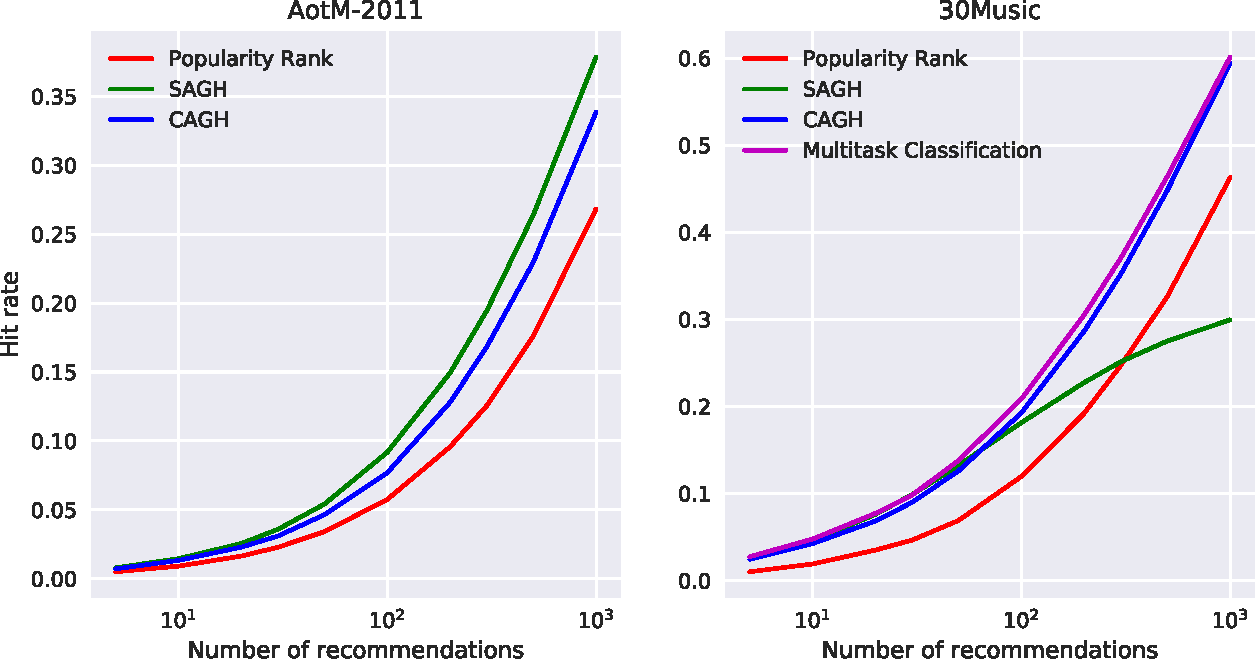
\includegraphics[width=\linewidth]{fig/hitrate-plgen1.pdf}
\caption{Hit rates given known users.}
\end{figure}

\begin{table}[!h]
\centering
\caption{Performance (given new user) in terms of R-Precision ($\times 10^2$)}
\label{tab:perf_plgen2_r-precision}
\begin{tabular}{l*{4}{c}*{4}{c}}
\toprule
Method     & AotM-2011 & 30Music \\
\midrule
Popularity Rank &     $1.3$ &   $2.1$ \\
Top10 SAGH &     $1.2$ &   $2.0$ \\
Top10 CAGH &     $1.2$ &   $2.0$ \\
Multitask Classification &       N/A &   $2.1$ \\
Multitask Ranking &       N/A &     N/A \\
\bottomrule
\end{tabular}
\end{table}


\begin{figure}[!h]
\centering
%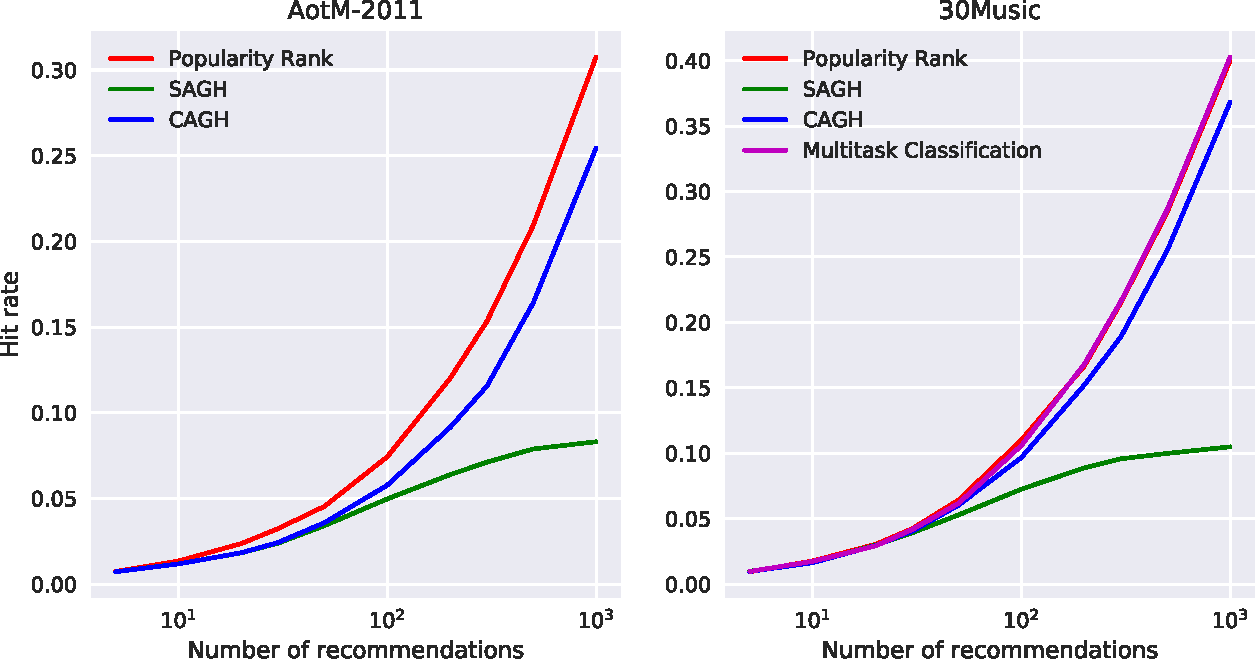
\includegraphics[width=\linewidth]{fig/hitrate-plgen2.pdf}
\caption{Hit rates given new users.}
\end{figure}



\subsection{New song recommendation}
\label{ssec:newsongrec}

We hold 5,000 and 10,000 of the latest released songs for test in the 30Music and AotM-2011 dataset, respectively.
For each song in test set, we predict whether it will be included in a given playlist.
As a remark, the set of users are the same for training and test, 
and playlists where every song is in test set are removed during training,
further, we test for playlists that has songs in both training and test set.
Table~\ref{tab:stats_newsongrec} summarises the statistics of the two dataset used for this task.

To tune hyper-parameters, we hold a subset of songs in training set as the validation set, 
which is constructed using the same approach as the test test.

\begin{table}[!h]
\centering
\caption{Statistics of dataset for new song recommendation}
\label{tab:stats_newsongrec}
%\resizebox{\linewidth}{!}{
\small
\begin{tabular}{lrrr}
\toprule
Dataset   & \#Playlists & \#Songs (train) & \#Songs (test) \\
\midrule
30Music   & 8,215       & 40,468          & 5,000 \\
AotM-2011 & 19,504      & 104,428         & 10,000 \\
\bottomrule
\end{tabular}
%}
\end{table}

\paragraph{Baselines}
\begin{itemize}
\item Logistic Regression: independently learn a logistic regression classifier for each playlist.
\item Shortest First: for each new song, recommend it to the shortest playlists in consideration.
\item Longest First: for each new song, recommend it to the longest playlists in consideration.
\item Ranking songs by the popularity of its artist and recommend the top-k, considering all songs in music collection.
\item Similar to the above method, but only considering songs of artists that the given user used to listen. 
(Note this baseline require the user is given).
\end{itemize}

\begin{table}[!h]
\centering
\caption{Empirical results (R-Precision $\times 10^3$)}
%\resizebox{\linewidth}{!}{
\small
\begin{tabular}{l|cccc}
\toprule
{}            & & & & BR \\
\midrule
AotM-2011     &  &  &  & 0.92 \\
30Music       &  &  &  & 7.24 \\
\bottomrule
\end{tabular}
%}
\end{table}


